\documentclass{article}
\usepackage{hyperref}
\usepackage{listings}
\usepackage{color}
\usepackage{subfigure}
\usepackage{geometry}
\usepackage{graphicx}
\usepackage{amsmath}
\geometry{margin=1in}

\newcommand\TODO[1]{\textcolor{red}{TODO: #1}}

\newcommand\header[2]{
    \begin{center}
        {\large
        UCSD CSE 272 Assignment #1: \\
        \vspace{0.3cm}
        \Large
        #2}
    \end{center}
}

\definecolor{dkgreen}{rgb}{0,0.6,0}
\definecolor{gray}{rgb}{0.5,0.5,0.5}
\definecolor{mauve}{rgb}{0.58,0,0.82}
\lstset{frame=tb,
        aboveskip=3mm,
        belowskip=3mm,
        showstringspaces=false,
        columns=flexible,
        basicstyle={\small\ttfamily},
        numbers=none,
        numberstyle=\tiny\color{gray},
        keywordstyle=\color{blue},
        commentstyle=\color{dkgreen},
        stringstyle=\color{mauve},
        breaklines=true,
        breakatwhitespace=true,
        tabsize=2
}

\begin{document}

\header{0}{Introduction to the \textbf{lajolla} Renderer}

For most parts of this course, we will use a custom physically-based renderer called \textbf{lajolla}.\footnote{Many renderers are named over a location. For example, Weta Digital's renderer \emph{Manuka}'s name comes from the Manuka street in front of Weta digital's main site. Pixar's rendering algorithm Reyes comes from Point Reyes in California.} This document presents the design of the lajolla renderer. Your first homework is to read through this document, and build and run the renderer, and look at the renderer's code. This homework is not graded. However, since lajolla is still at its early stage, we expect it to have a few bugs. If you find or fix any bugs in lajolla throughout the course, you will get extra points!

Lajolla is a \emph{physically-based} renderer. It takes a 3D scene description (camera, lights, geometry, materials, etc) and input, and produces an image by simulating how photons emitted from the light sources scattered in the scene and eventually reach the camera. This is how modern visual effects, and many video games produce stunning and realistic images. Apart from movies and games, physically-based rendering is also used in augmented reality, architectural visualization, daylight simulation, product visualization, medical imaging, computer vision, autonomous driving and more. A startup \href{https://www.luxion.com/}{Luxion} from a UCSD faculty \href{http://graphics.ucsd.edu/~henrik/}{Henrik Jensen} is about building physically-based renderers and use them for many applications above.

\section{Building and running lajolla}
\begin{figure}[h]
    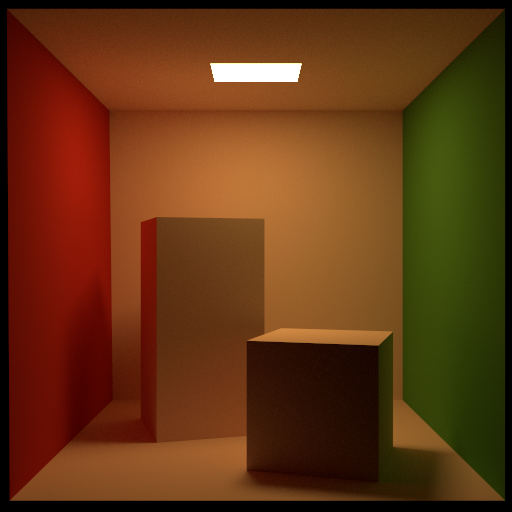
\includegraphics[width=0.24\linewidth]{imgs/cbox.png}
    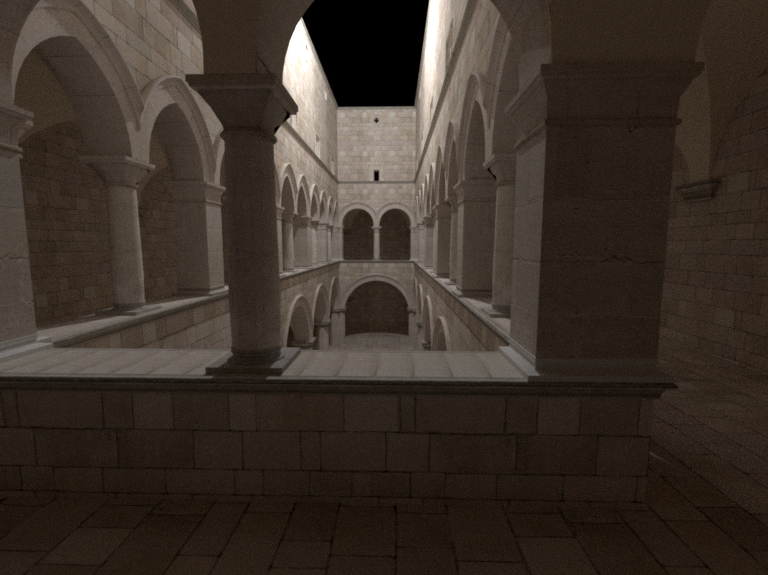
\includegraphics[width=0.24\linewidth]{imgs/sponza.png}
    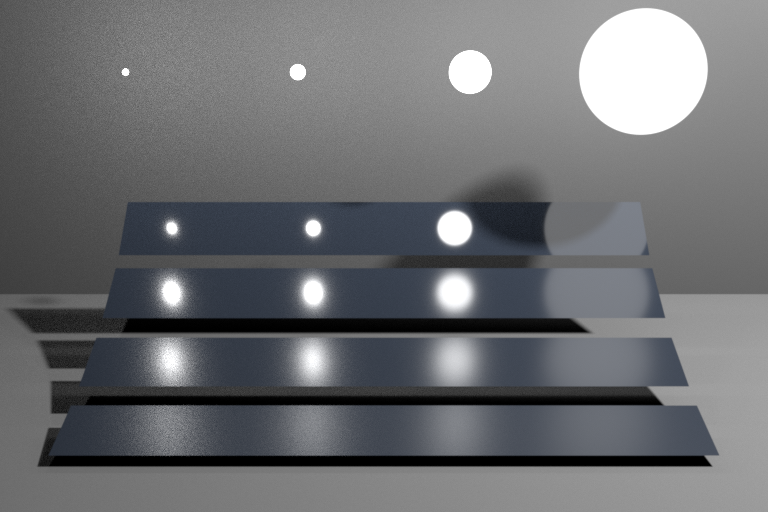
\includegraphics[width=0.24\linewidth]{imgs/veach_mis.png}
    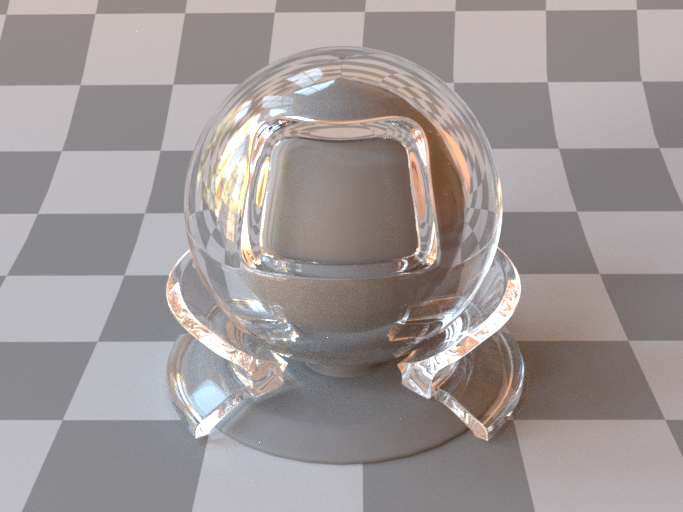
\includegraphics[width=0.24\linewidth]{imgs/matpreview.png}
    \caption{Images you can render using lajolla.}
    \label{fig:gallery}
\end{figure}

Before we started, let's try to clone, build the code and run it. Lajolla does not require you to download any external libraries (hopefully). While we do rely on many 3rdparty libraries, we only use lightweight header-only ones that can be easily included and do not complicate the build systems. To clone the codebase, do

\begin{lstlisting}[language=bash]
  git clone https://github.com/BachiLi/lajolla_public
\end{lstlisting}

We use \href{https://cmake.org/}{CMake} as our build system. To build, on a Unix-like system, do the following from the \lstinline{lajolla_public} directory:

\begin{lstlisting}[language=bash]
  mkdir build
  cd build
  cmake ..
  make -j
\end{lstlisting}

On Windows, latest visual studio supports directly using CMake as project files.\footnote{\url{https://docs.microsoft.com/en-us/cpp/build/cmake-projects-in-visual-studio?view=msvc-170}} Alternatively, you can use CMake's graphical user interface downloaded from CMake's website. However, we have received reports that lajolla can crash on Windows machines. You might want to consider using Windows Subsystems for Linux to use a Unix-like systems for building and running lajolla (or you can help us fixing issues on Windows and get extra points!). 

Once lajolla is built, you can try to render some images in the \lstinline{scenes} directory. Try
\begin{lstlisting}[language=bash]
  ./lajolla ../scenes/cbox/cbox.xml
\end{lstlisting}

After the reading is done, you will see an image file \lstinline{image.exr} appeared in your working directory. EXRs are \emph{high-dynamic range images}\footnote{\url{https://en.wikipedia.org/wiki/High_dynamic_range}} and require a different image viewer. We recommend viewing it using HDRView\footnote{\url{https://github.com/wkjarosz/hdrview}} or Tev\footnote{\url{https://github.com/Tom94/tev}}. You should be able to see images like the ones in Figure~\ref{fig:gallery} (maybe noiser, since the default settings for these scenes use a smaller number of light simulation samples compared to the ones in the figure).

The scene format in lajolla follows the Mitsuba scene format, where you can read the documentation \href{https://www.mitsuba-renderer.org/releases/current/documentation.pdf}{here}. The scene files are human readable, so by just looking at those files should gives you a reasonable idea.

\section{Design philosophy}

Lajolla mostly follows the design of other existing physically-based renderers, such as \href{https://github.com/mmp/pbrt-v3/}{pbrt} or \href{http://www.mitsuba-renderer.org/}{Mitsuba}. It however follows a few different designs:

\paragraph{Minimalism.} While already sophisticated, lajolla is much less feature complete compared to pbrt or Mitsuba. This is the main reason we are inventing our own renderer instead of adopting existing ones. This is mostly for educational purpose: if all the features are implemented, there won't be any homeworks. : )

\paragraph{Clarity and simplicity over performance.} Lajolla does not try to become the fastest renderer in the world. The focus is on education. For example, by default lajolla uses double for most floating point computation and does not explicitly vectorize over any computation.

\paragraph{Portability to GPU.} Lajolla does not run on GPUs. The goal of this course is to teach the foundation of modern physically-based rendering instead of all the implementation details. That being said, given that GPU rendering is going to be increasingly important even in the offline rendering world, we need to learn how to build a renderer that is more portable to GPUs. Most functions and data structures in lajolla should be directly usable in CUDA or OpenCL code, given small amount of modification. Lajolla avoids deeply nested hierarchical data structures and also avoids heap allocation in the inner loop as much as possible.

\paragraph{Modern C++.} Lajolla uses modern C++ features extensively (fortunately, it does not use template metaprogramming extensively). This means it prefers value semantics over reference semantics:
\begin{lstlisting}[language=C++]
  std::tuple<int, int> foo(int x); // preferred
  void bar(int x, int *y, int *z); // less preferred
  std::optional<float> foo2(const float &x); // preferred
  bool bar2(const float &x, float *out); // less preferred
\end{lstlisting}
We do not just \lstinline{auto} that often, since I am still not convinced that it would not hurt code readability.

\paragraph{Variant-based polymorphism.} Perhaps the biggest different on the surface between lajolla and most other (CPU-based) renderers is how it implements polymorphism. In rendering, the same rendering code would need to handle different materials, lights, cameras, and etc. Most renderers adopt a heavily object-oriented design with classes and inheritance. While this is an acceptable approach, the hierarchical vtable pointers make the whole scene data structure very difficult to convert to GPU. I also personally just do not think OOP is a good idea\footnote{see "Object-Oriented Programming is Bad" from Brain Will \url{https://www.youtube.com/watch?v=QM1iUe6IofM}}. To support polymorphism, we use a modern C++ feature \lstinline{std::variant}. It is essentially a \emph{tagged union} (or a \emph{sum type} if you are functional guru): a C union with a member indicating which type it is. Read more about it \href{https://www.cppstories.com/2020/04/variant-virtual-polymorphism.html/}{here}. Another renderer \href{visionaray}{https://github.com/szellmann/visionaray} also adopts a similar approach.

Below we will take a whirlwind tour over the basics of physically-based rendering and how they are implemented in lajolla.

\section{Rendering equation(s)}
\begin{figure}[h]
    \centering
    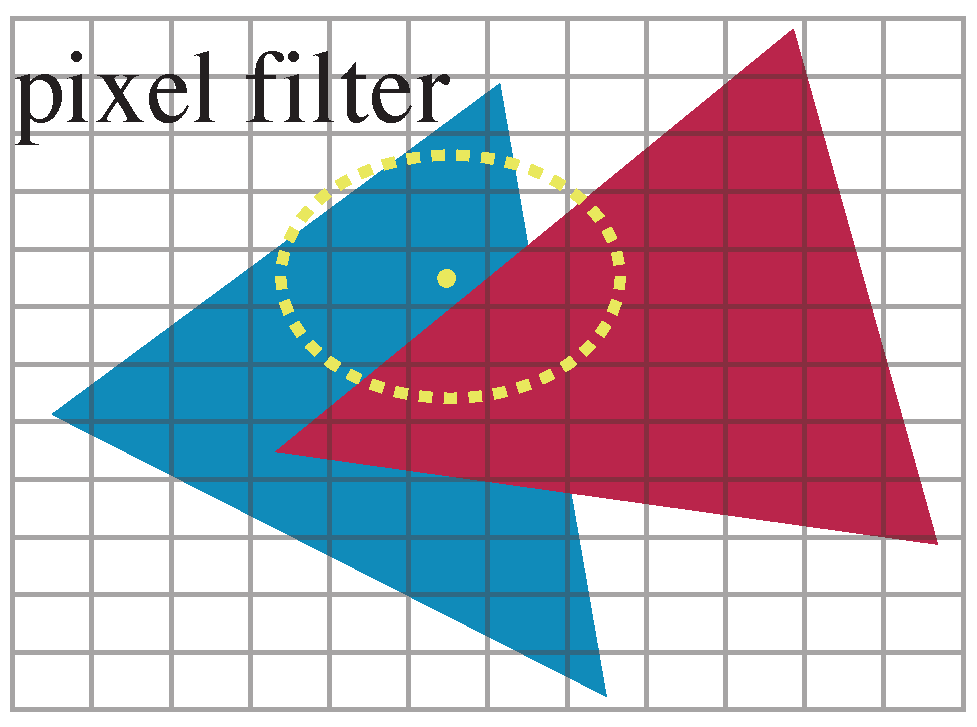
\includegraphics[width=0.4\linewidth]{imgs/pixel_filter.pdf}
    
\includegraphics[width=0.4\linewidth]{imgs/antialiasing.pdf}
    \caption{To reconstruct the continuous scene from the discrete pixel samples, the color of a pixel is reconstructed by integrating over a \emph{pixel filter}.}
    \label{fig:pixel_filter}
\end{figure}

\begin{figure}[h]
    \centering
    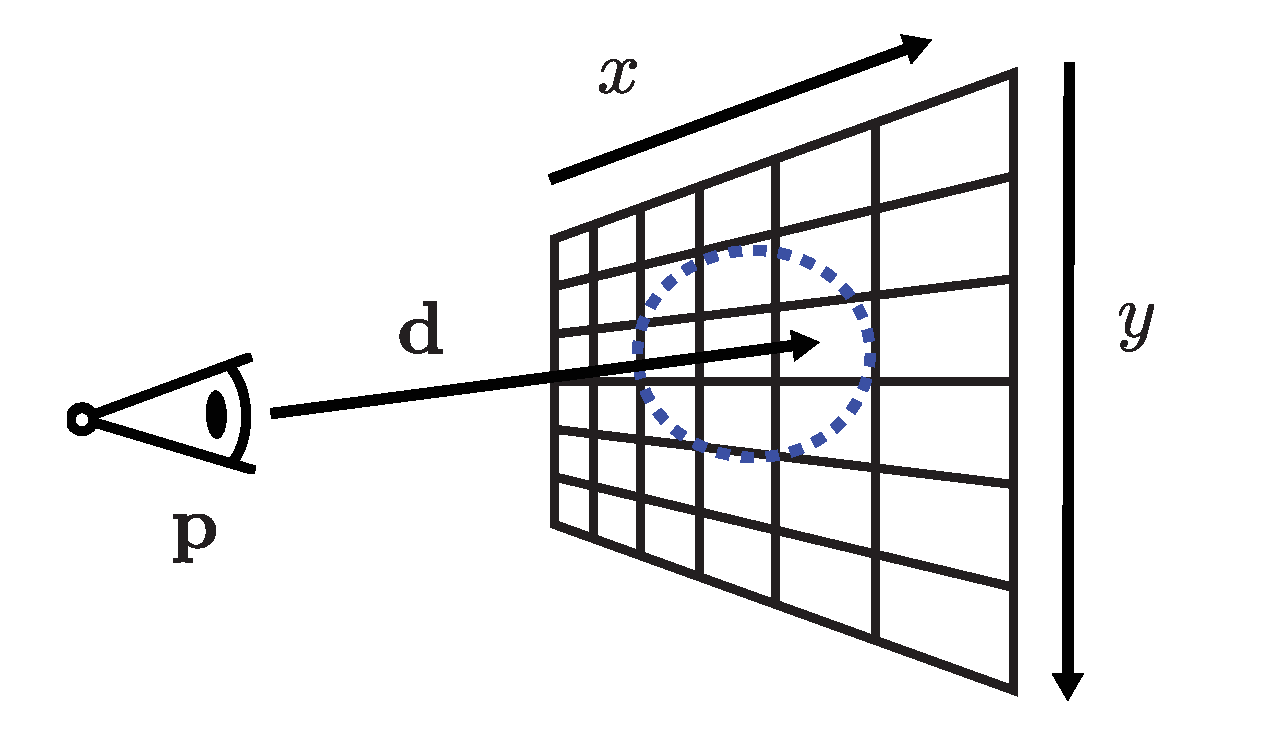
\includegraphics[width=0.4\linewidth]{imgs/camera.pdf}
    \caption{Camera configuration and pixel filtering.}
    \label{fig:camera}
\end{figure}

How does lajolla, or many other modern physically-based renderer compute the color for each pixel? They do this by \emph{integrating} all lights that goes through a pixel. Note that a pixel is not a infinitesimal point, not is it a little square~\cite{Smith:1995:PLS}. \textbf{A pixel is a reconstruction filter over an image function at a certain locatio} (Figure~\ref{fig:pixel_filter}). Mathematically, a pixel $I_{x, y}$'s color is written as an filtering integral:
\begin{equation}
    I_{x, y} = \iint_{D} k(x', y') L(\mathbf{p}, \mathbf{d}(x + x', y + y')) \mathrm{d}x\mathrm{d}y,
    \label{eq:pixel_filter}
\end{equation}
where $k$ is the \emph{filter kernel}, $D$ is the \emph{support} of the filter kernel (the pixel location where its value is non-zero), and $L(\mathbf{p}, \mathbf{d})$ is the radiance at point $\mathbf{p}$, received from direction $\mathbf{\omega}$ where the direction is pointing outwards from $\mathbf{p}$. In our case, $\mathbf{p}$ is the position of the camera, and $\mathbf{\omega}$ is the direction between the camera position and the points on the film (Figure~\ref{fig:camera}).

Now we have three questions: 1) what is the filter kernel $k$? 2) what is the radiance $L$?, and 3) how do we evaluate this integral on a computer? For 1), we will discuss a bit more in Section~\ref{sec:pixel_filter}, but for now you can think of it as something like a 2D Gaussian. For 3), these integrals typically do not have closed-form solutions,\footnote{There are rendering algorithms that based on closed-form solutions of these integrals. Some radiosity algorithms~\cite{Schroder:1993:OFF} make use of closed-form solutions, for example. Also check out the excellent paper from Heitz et al.~\cite{Heitz:2016:RPS}} so we need to \emph{discretize} these integrals:
\begin{equation}
    \int_{D} F(x) dx \approx \frac{1}{N} \sum_{i=1}^{N} F(x_i),
    \label{eq:discretization}
\end{equation}
where $x_i$ are samples in uniform measures drawn from the domain $D$. When $x_i$ are random samples, this is called \emph{Monte Carlo} integration.\footnote{Monte Carlo integration was first invented for numerical simulation of nuclear weapons. Nicholas Metropolis, a member of the Manhatton Project, suggested the name to the simulation guy Stanislaw Ulam since Ulam's uncle likes to go to Monte Carlo for gambling.} However, $x_i$ do not need to be random. It can be determinisic samples that just somewhat uniformly cover the domain. When $x_i$ are deterministic, this approximation is often called \emph{quadrature} or \emph{cubature}. There is another class of deterministic integration methods called \emph{Quasi Monte Carlo} methods, which is based on the idea of carefully placing samples to make sure they are not far away from each other. We will cover these in the class if time permits.

\begin{figure}[h]
    \centering
    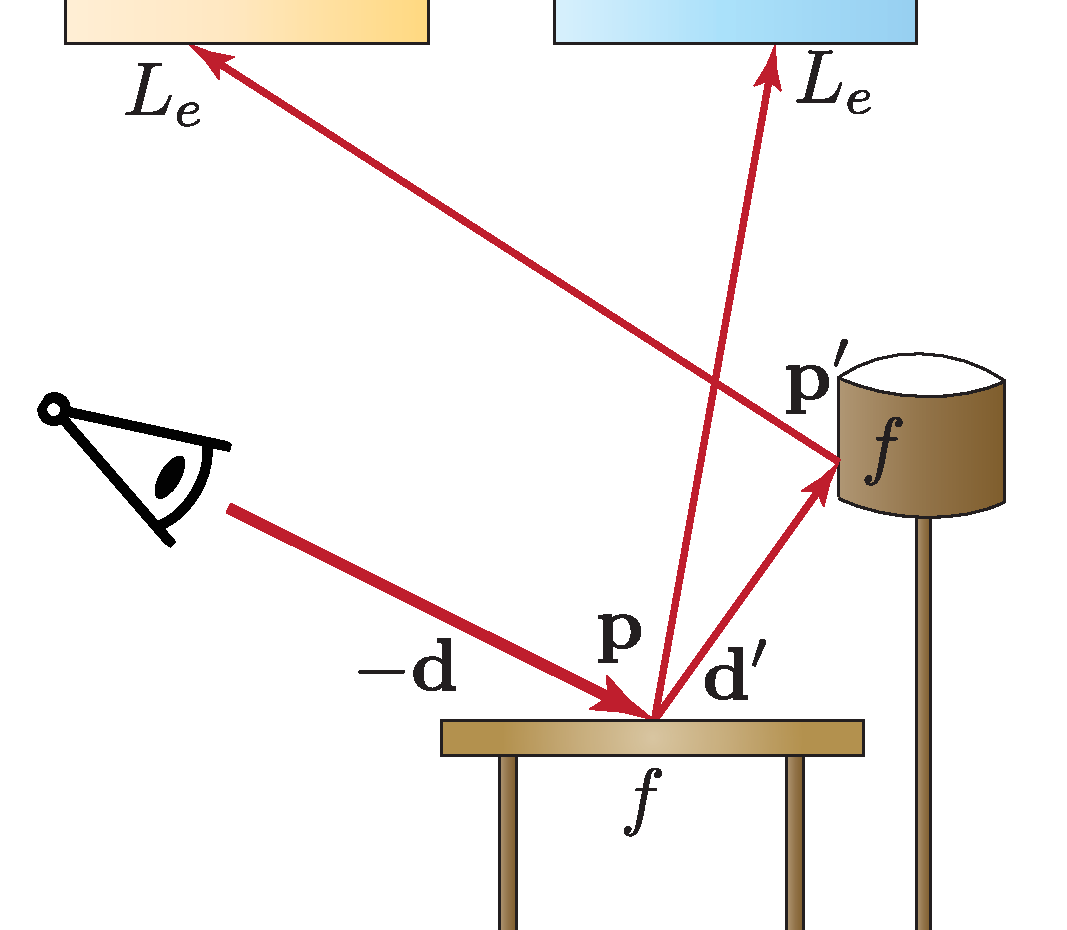
\includegraphics[width=0.4\linewidth]{imgs/pathtracing.pdf}
    \caption{The illustration of the rendering equation.}
    \label{fig:pathtracing}
\end{figure}

We are still left with Q2: what is the radiance $L$? In this class, we are mostly dealing with objects that are larger than the wavelength of lights. So under Newtonian optics, the radiance is simply the radiance $L_i$ at the object we see:
\begin{equation}
    L(\mathbf{p}, \mathbf{\omega}) = L_i(\mathbf{p}', -\mathbf{\omega}),
\end{equation}
where $\mathbf{p}'$ is the point the direction $\mathbf{d}$ intersect with the scene. Then -- what is $L_i$? An object is lit by a light source. However, as photons scatter between objects, a photon can first hit object A before it hits object B. Therefore we need to recursively consider all objects in the scene:
\begin{equation}
    L_i(\mathbf{p}, \mathbf{\omega}) = L_e(\mathbf{p}, \mathbf{\omega}) + \int_{\Omega} f(\mathbf{p}, \mathbf{\omega}, \mathbf{\omega}') |\mathbf{n}_{\mathbf{p}} \cdot \mathbf{\omega}'| L_i(\mathbf{p}', -\mathbf{\omega}') \mathrm{d} \mathbf{\omega},
    \label{eq:rendering_equation}
\end{equation}
where $L_e$ is the \emph{emission} at $\mathbf{p}$ towards direction $\mathbf{\omega}$, $\Omega$ is a spherical domain around point $\mathbf{p}$, $f$ is the reflectance of the object at point $p$ from direction $\mathbf{\omega}'$ to $\mathbf{\omega}$, $\mathbf{p}'$ is the point intersected by the ray $(\mathbf{p}, \mathbf{\omega}')$, and $n_{p}$. $f$ is often called the Bidirectional Scattering Distribution Function (BSDF) -- when the material is transmissive, it's called the Bidirectional Transmission Distribution Function (BTDF), and when it is reflective, it's called the Bidirectional Reflectance Distribution Function (BRDF) (I know, it's confusing). See Figure~\ref{fig:pathtracing} for an illustration. The measure $\mathrm{d} \mathbf{\omega}_{\bot}'$ is the \emph{solid angle}: the infinitesimal area on a unit sphere. Equation~\ref{eq:rendering_equation} is often called the \emph{rendering equation}~\cite{Kajiya:1986:RE}.

This recursive integral, combined with the integral discretization (Equation~\ref{eq:discretization}), gives us an rendering algorithm. We start from a pixel $(x, y)$, and sample a pixel offset $(x', y')$ to estimate the pixel filter integral (Equation~\ref{eq:pixel_filter}). Next, to estimate $L_i$, we sample a direction $\mathrm{d}'$, hit point $\mathbf{p}'$, multiply by $f$, and add $L_e$ whenever we hit a light source. In lajolla, the \lstinline{path_tracing} function in \lstinline{path_tracing.h} implements a slightly more sophisticated version of this. In below we describe those improvements.

\subsection{Importance sampling}
The naive algorithm above is correct, but can be inefficient. Consider a special case of the rendering equation, where we only recurse once:
\begin{equation}
    L_i(\mathbf{p}, \mathbf{d}) = L_e(\mathbf{p}, \mathbf{\omega}) + \int_{\Omega} f(\mathbf{p}, \mathbf{\omega}, \mathbf{\omega}') |\mathbf{n}_{\mathbf{p}} \cdot \mathbf{\omega}'| L_e(\mathbf{p}', -\mathbf{\omega}') \mathrm{d} \mathbf{\omega}.
\end{equation}
The only difference is that instead of $L_i$ in the integral that recursively integrate over all the other surfaces, we only consider the light source contribution $L_e$. Remember that we approximate the integral using a discrete sum. Suppose we randomly sample a direction on a sphere:
\begin{equation}
  \int_{\Omega} f(\mathbf{p}, \mathbf{\omega}, \mathbf{\omega}') |\mathbf{n}_{\mathbf{p}} \cdot \mathbf{\omega}'| L_e(\mathbf{p}', -\mathbf{\omega}') \mathrm{d} \mathbf{\omega} \approx \frac{1}{N} \frac{1}{\frac{1}{4 \pi}} \sum_{i}^{N} f(\mathbf{p}, \mathbf{\omega}, \mathbf{\omega}_i') |\mathbf{n}_{\mathbf{p}} \cdot \mathbf{\omega}'| L_e(\mathbf{p}', -\mathbf{\omega}_i').
\end{equation}
The $\frac{1}{\frac{1}{4\pi}}$ factor accounts for the uniform measure on an unit sphere. The variance of this sum can be really high if $N$ is not large enough: firstly, not every surface in the scene emits light, so only a small fraction of samples would have non-zero $L_e$. Secondly, our sampling does not take the BSDF $f$ into consideration: $f$ can have high variation between different samples.

Fortunately, there is a way to make this sampling more efficient. The key is to apply a change of variable to our integral. Let's focus on the emission $L_e$ first. Instead of blindly sampling a direction on the sphere, we can directly pick a point on the light source, then choose a direction towards that point. So instead of integrating over the direction $\mathbf{\omega}$, we apply a change of variable to instead integrate over the points $\mathbf{p}$ that emit lights:
\begin{equation}
    \int_{\Omega} f(\mathbf{p}, \mathbf{\omega}, \mathbf{\omega}') |\mathbf{n}_{\mathbf{p}} \cdot \mathbf{\omega}'| L_e(\mathbf{p}', -\mathbf{\omega}') \mathrm{d} \mathbf{\omega} =
    \int_{E} f(\mathbf{p}, \mathbf{\omega}, \mathbf{\omega}'(\mathbf{p}')) |\mathbf{n}_{\mathbf{p}} \cdot \mathbf{\omega}'| L_e(\mathbf{p}', -\mathbf{\omega}') G(\mathbf{p}, \mathbf{p}') \mathrm{d} \mathbf{p}',
\end{equation}
where $E$ is the area of all light sources, and $G$ is the Jacobian of the variable reparametrization (often called the \emph{geometry term}). Using some geometry insights, we can derive that $G(\mathbf{p}, \mathbf{p}') = \frac{|\mathbf{n}_{\mathbf{p}'} \cdot \mathbf{d}'|}{\|\mathbf{p} - \mathbf{p}'\|^2} V(\mathbf{p}, \mathbf{p}')$, where $V(\mathbf{p}, \mathbf{p}')$ is the \emph{visibility function} where $V=1$ if $\mathbf{p}$ can see $\mathbf{p}'$ and $V=1$ if they are occluded. Intuitively, $G$ is the area ratio of an infinitesimal area projected onto an unit sphere.

When the light source is visible for most of the time, the discretization of the second integral is much more efficient at locating lights since we focus on the domain $E$ instead of the whole spherical domain.

We can similarly account for the BSDF $f$ and the cosine $|\mathbf{n}_{\mathbf{p}} \cdot \mathbf{\omega}'|$ using a similar change of variable trick. This change of variable is often called \emph{importance sampling}.

In general, for a (potentially multi-dimensional) integral $\int g(x) \mathrm{d}x$, we can rewrite it using a change of variable $y = T(x)$, where $T$ is an invertible function. This gives us $\int g(T^{-1}(y)) \frac{1}{|\frac{\mathrm{d}y}{\mathrm{d}x}|} \mathrm{d}y$, where $|\frac{\mathrm{d}y}{\mathrm{d}x}|$ is the Jacobian of the mapping $T$. If we discretize the new integral using uniform samples $y_i$, then we can see the new discretization as drawing samples $x_i = T^{-1}(y_i)$, evaluate $g(x_i)$, then weight them with the inverse of the Jacobian $|\frac{\mathrm{d}y}{\mathrm{d}x}|$ (as opposed to drawing $x_i$ as uniform samples and weight them with $1$). The Jacobian can be seen as the \emph{probability density function} of the samples $x_i = T^{-1}(y_i)$ (since the probability density function needs to integrate to $1$, we are essentially applying a change of variable for that integral too). 

In lajolla, the \lstinline{sample_light} and \lstinline{sample_point_on_light} functions implement the light source sampling strategy above. \lstinline{sample_light} pick a light source (from many) proportional to their relative powers, and \lstinline{sample_point_on_light} pick a point on the selected light source. \lstinline{light_pmf} and \lstinline{pdf_point_on_light} are the probability density (or probability mass function in the case of discrete distributions) of the corresponding sampling operations. Similarly, \lstinline{sample_bsdf} samples a direction that is proportional to $f$, and \lstinline{pdf_sample_bsdf} is the corresponding probability density.

\subsection{Multiple importance sampling}

If we have multiple change of variables we want to apply (e.g., sampling from lights and sampling from BSDFs), how do we combine them? One (inefficient) way to do this is to combine them by averaging the results. For example, for an integral $\int g(x) \mathrm{d}x$, we can apply $y = T_1(x)$ and $z = T_2(x)$, and evaluate $\frac{g(x(y_i))}{
\frac{\mathrm{d}T_1}{\mathrm{d}x}|}$ and $\frac{g(x(z_i))}{|\frac{\mathrm{d}T_2}{\mathrm{d}x}|}$. We can approximate the integral as
\begin{equation}
\frac{1}{N} \sum
\frac{1}{2} \frac{g(x(y_i))}{|\frac{\mathrm{d}T_1}{\mathrm{d}x}(x(y_i))|} + 
\frac{1}{2} \frac{g(x(z_i))}{|\frac{\mathrm{d}T_2}{\mathrm{d}x}(x(z_i))|}.
\end{equation}

This is, however, not a great idea. If one of our sampling transformation has high variance, even if the other one achieves zero variance, this resulting estimator would still have very high variance.

Eric Veach made a breakthrough in physically-based rendering by figuring out how we combine different estimators~\cite{Veach:1995:OCS}. The idea is to apply higher weight for the \emph{better} estimator. How do we know which estimator is better? We look at the Jacobian $|\frac{\mathrm{d}T}{\mathrm{d}x}(x)|$, or equivalently the probability density: if the Jacobian is high, that means that our sampling strategy has high sampling density around $x_i$ -- which means it's more efficient around that area. We can weight the samples using the corresponding Jacobian:
\begin{equation}
\frac{1}{N} \sum
\frac{|\frac{\mathrm{d}T_1}{\mathrm{d}x}(x(y_i))|}{|\frac{\mathrm{d}T_1}{\mathrm{d}x}(x(y_i))| + |\frac{\mathrm{d}T_2}{\mathrm{d}x}(x(y_i))|}
\frac{g(x(y_i))}{|\frac{\mathrm{d}T_1}{\mathrm{d}x}(x(y_i))|} + 
\frac{|\frac{\mathrm{d}T_2}{\mathrm{d}x}(x(z_i))|}{|\frac{\mathrm{d}T_1}{\mathrm{d}x}(x(z_i))| + |\frac{\mathrm{d}T_2}{\mathrm{d}x}(x(z_i))|}
\frac{g(x(z_i))}{|\frac{\mathrm{d}T_2}{\mathrm{d}x}(x(z_i))|}.
\end{equation}
Alternatively, Veach also proposed another weight called the \emph{power heuristics} that put even more emphasis on strategies with high Jacobian values:
\begin{equation}
\frac{1}{N} \sum
\frac{|\frac{\mathrm{d}T_1}{\mathrm{d}x}(x(y_i))|^2}{|\frac{\mathrm{d}T_1}{\mathrm{d}x}(x(y_i))|^2 + |\frac{\mathrm{d}T_2}{\mathrm{d}x}(x(y_i))|^2}
\frac{g(x(y_i))}{|\frac{\mathrm{d}T_1}{\mathrm{d}x}(x(y_i))|} + 
\frac{|\frac{\mathrm{d}T_2}{\mathrm{d}x}(x(z_i))|^2}{|\frac{\mathrm{d}T_1}{\mathrm{d}x}(x(z_i))|^2 + |\frac{\mathrm{d}T_2}{\mathrm{d}x}(x(z_i))|^2}
\frac{g(x(z_i))}{|\frac{\mathrm{d}T_2}{\mathrm{d}x}(x(z_i))|}.
\end{equation}

Veach made more justification of the method in his paper (which I highly recommend you to read!). However note that these are ultimately ``heuristics'', and they can be suboptimal in certain cases. Finding better multiple importance sampling weights is an active research area.

lajolla uses the power heuristics for combining different strategies.

\paragraph{The path-space integral.} The rendering equation above is a recursive equation, and while recursion is cool, it's often easier to analyze and understand its structure if we can flatten it to a more iterative form. By expanding the recursion, we see the following pattern
\begin{equation}
    L_i = L_e + f * L_e + f * f * L_e + \dots.
\end{equation}
We notice that we are essentially tracing \emph{light paths} with different number of vertices. For light paths with two vertices: one at the camera position and one at a light source, we only need to compute $L_e$. For light paths with three vertices, we need to account for one scattering event and multiply $f$. If we define a light path with a sequence of directions: $\mathbf{D} = ((x', y'), \mathbf{d}_1, \mathbf{d}_2, \dots)$, then we can define a \emph{path contribution function} $f_d$ to compute the contribution of that single light path. From above, we can see that
\begin{equation}
    f_d(\mathbf{D}) = k(x', y') f(\mathbf{p}_1, \mathbf{d}_0(x', y'), \mathbf{d}_1) f(\mathbf{p}_2, \mathbf{d}_1, \mathbf{d}_2) \dots L_e(\mathbf{p}_N, \mathbf{d}_N).
\end{equation}
(I might have get some signs wrong but don't worry about it.)

We can then rewrite the rendering integral as
\begin{equation}
    I_{x, y} = \int f_d(\mathbf{D}) \mathrm{d} D(\mathbf{d}),
\end{equation}
where the measure $D(\mathbf{d})$ is the product of solid angle of the path directions $\mathbf{d}_i$.

A path can also be written in many different forms. A very convienent form is to define the path as a sequence of positions, as opposed of directions: $\mathbf{P} = (\mathbf{p}_0, \mathbf{p}_1, \mathbf{p}_2, \dots)$. While these two forms are equivalent, this again is a change of variable. The new path contribution function $f_p(\mathbf{P})$ is:
\begin{equation}
    f_p(\mathbf{P}) = k((x', y')(\mathbf{p}_0, \mathbf{p_1})) G_0(\mathbf{p}_0, \mathbf{p}_1) f(\mathbf{p}_1, \mathbf{d}_0, \mathbf{d}_1)G(\mathbf{p}_1, \mathbf{p}_2) f(\mathbf{p}_2, \mathbf{d}_1, \mathbf{d}_2) \dots G(\mathbf{p}_{N-1}, \mathbf{p}_{N}) L_e(\mathbf{p}_N, \mathbf{d}_N),
\end{equation}
where $G$ is again the geometry term that accounts for the Jacobian. The first geometry term $G_0$ is slightly more complicated as it is the Jacobian between $\mathbf{p}_1$ and pixel integral variables $x', y'$. We don't need it here yet, so don't worry about it.

This path integral enables a more principled way to think about rendering algorithms. For example, we do not need to always trace paths from the cameras. We can trace paths from lights and it still gives us a valid light path. We can even just randomly sample spatial location to construct a sequence of positions $\mathbf{p}$.

\section{Camera}

\subsection{Pixel filter}
\label{sec:pixel_filter}

\section{Materials}

\subsection{Textures and filtering}

\section{Lights}

\section{Geometry}

\section{Utilities}

\subsection{Vectors}

\subsection{Matrices}

\subsection{Frame}

\subsection{Color}

\subsection{Parallelization}

\subsection{Random number generation}

\bibliographystyle{plain} % We choose the "plain" reference style
\bibliography{refs} % Entries are in the refs.bib file

\end{document}
